\documentclass{article}

\usepackage{polski}
\usepackage[margin=1in]{geometry}
\usepackage[parfill]{parskip}
\usepackage{amsmath}
\usepackage{graphicx}
\usepackage{caption}
\usepackage{siunitx}
\usepackage[table,xcdraw]{xcolor}
\usepackage{hyperref}
\usepackage[T1]{fontenc}
\usepackage{comment}
\usepackage{float}

\begin{document}

\begin{center}
\bgroup
\def\arraystretch{1.5}
\begin{tabular}{|c|c|c|c|c|c|}
	\hline
	EAIiIB & \multicolumn{2}{|c|}{\begin{tabular}{@{}c@{}}Stanisław Borowy \\ Maciej Bobrek \end{tabular}} & Rok II & Grupa 1 & Zespół 5 \\
	\hline
	\multicolumn{3}{|c|}{\begin{tabular}{c}Temat:\\Indukcyjność wzajemna \end{tabular}} & 
	\multicolumn{3}{|c|}{\begin{tabular}{c}Numer ćwiczenia: \\44 \end{tabular}} \\
	\hline
	\begin{tabular}{@{}c@{}}Data wykonania \\ 01.01.2023 \end{tabular} & \begin{tabular}{@{}c@{}}Data oddania \\ 02.01.2023 \end{tabular} & 
	\begin{tabular}{c}Zwrot do popr.\\\phantom{data} \end{tabular} & \begin{tabular}{c}Data oddania\\\phantom{data}\end{tabular} &
	\begin{tabular}{c}Data zaliczenia\\\phantom{data}\end{tabular} & \begin{tabular}{c}Ocena\\\phantom{ocena}\end{tabular} \\[4ex]
	\hline
\end{tabular}
\egroup
\end{center}

\section{Cel ćwiczenia}
Pomiar współczynnika indukcji wzajemnej dwóch cewek sprzężonych ze sobą magnetycznie, dla różnych
wzajemnych położeń tych cewek. Wpływ rdzenia magnetycznego na indukcyjność własną i wzajemną.

\section{Wstęp teoretyczny}
Wytwarzane przez parę cewek pola magnetyczne mogą na siebie
oddziaływać.
Zjawisko to nazywamy \emph{sprzężeniem magnetycznym}, a wielkość je
charakteryzującą \emph{indukcją wzajemną}. W celu wyznaczenia wzoru
indukcji wzajemnej dzielimy strumień pola magnetycznego $\phi$ na
dwie części:
\begin{enumerate}
    \item strumień główny $\phi_g$ -- część przenikającą przez drugą cewkę,
    \item strumień rozproszenia $\phi_s$ -- część nie obejmująca
    drugiej cewki.
\end{enumerate}
Tak więc rozkład $\phi$ wyrażamy wzorem
\begin{align*}
    \phi = \phi_g + \phi_s.
\end{align*}
Stosunek strumienia magnetycznego skojarzonego z danym uzwojeniem do prądu $i$, który wywołuje ten
strumień, nazywamy \emph{indukcyjnością własną} $L$ uzwojenia i
wyrażamy ją wzorem
\begin{align*}
    L = \frac{N\phi}{i},
\end{align*}
gdzie $N$ jest liczbą zwojów cewki. Podobnie definiuje się indukcyjność
wzajemną dwóch cewek
\begin{align*}
    M = \frac{N_2\phi_{1g}}{i_1}. = \frac{N_1\phi_{2g}}{i_2}
    \label{eq:wzajemna}
\end{align*}
W powyższym wzorze indeksy dolne służą rozróżnieniu pomiędzy
dwiema cewkami.

Korzystając z podanych praw, da się wykazać, że
\begin{align}
    M = k\sqrt{L_1L_2},
\end{align}
gdzie $k$ nazywamy \emph{współczynnikiem sprzężenia}.

Pomiary $L$ tych samych cewek połączonych ze sobą przy zgodnym zwrocie
nawinięcia ($L_z$) i przeciwnym zwrocie nawinięcia ($L_p$) można wykorzystać w celu
obliczenia $M$ i $k$ następującymi wzorami

\begin{align}
    \label{eq:M}
    M = \frac{L_z - L_p}{4}\\
    \label{eq:k}
    k = \frac{M}{\sqrt{L_1L_2}}.
\end{align}

\pagebreak
\section{Aparatura}
Do wykonania ćwiczenia zespół użył 
\begin{enumerate}
    \item Dwie Cewki umieszczone na podstawce
    \item Prowadnica
    \item Amperomierz
    \item Miernik LCR
\end{enumerate}
Podane wyżej komponenty zostały połączone w następujący układ. Układ a przedstawia sprzężenie dodatnie, a układ b sprzężenie ujemne.

\begin{figure}[h!]
    \centering
    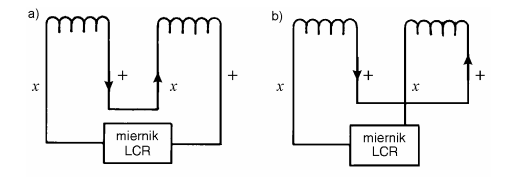
\includegraphics[scale=0.6]{cw44/układ.png}
    \caption{Schemat wykorzystanego układu pomiarowego}
\end{figure}
 Zespół wykonywał pomiary indukcyjności wypadkowej dla dodatniego i ujemnego sprzężenia cewek powietrznych zmieniając odległość cewek o 0,5 cm. 
 \section{Wyniki Pomiarów}
 Przed pomiarami zespół zmierzył indukcyjność własną obu cewek, dla małej $L_{1}$, a dla dużej $L_{2}$.\newline
 \begin{align*}
   L_1= 0,1 \si{H}
\end{align*}
\begin{align*}
    L_2= 3 \si{H}
\end{align*}
Następnie wykonano pomiary dla dodatniego sprzężenia cewek, a wyniki zebrano w tabeli \ref{tabe:1}
\begin{table}[!ht]
    \centering
    \begin{tabular}{|l|l|l|l|l|l|l|l|l|l|l|l|l|}
    \hline
        Lp. & 1 & 2 & 3 & 4 & 5 & 6 & 7 & 8 & 9 & 10 & 11 & 12 \\ \hline
        x[cm] & 3 & 3,5 & 4 & 4,5 & 5 & 5,5 & 6 & 6,5 & 7 & 7,5 & 8 & 8,5 \\ \hline
        L[H] & 3,43 & 3,4 & 3,39 & 3,38 & 3,35 & 3,3 & 3,3 & 3,27 & 3,25 & 3,22 & 3,2 & 3,18 \\ \hline
    \end{tabular}
    \caption{Wyniki pomiarów indukcyjności dla dodatniego sprzeżenia cewek}
    \label{tabe:1}
\end{table}

W kolejnym kroku wykonano pomiary dla ujemnego sprzężenia cewek, a wyniki zebrano w tabeli \ref{tabe:2}
\begin{table}[!ht]
    \centering
    \begin{tabular}{|l|l|l|l|l|l|l|l|l|l|l|}
    \hline
        Lp. & 1 & 2 & 3 & 4 & 5 & 6 & 7 & 8 & 9 & 10 \\ \hline
        x[cm] & 4 & 4,5 & 5 & 5,5 & 6 & 6,5 & 7 & 7,5 & 8 & 8,5 \\ \hline
        L[H] & 2,8 & 2,82 & 2,84 & 2,87 & 2,89 & 2,92 & 2,94 & 2,96 & 2,98 & 3 \\ \hline
    \end{tabular}
    \caption{Wyniki pomiarów indukcyjności dla ujemnego sprzeżenia cewek}
    \label{tabe:2}
\end{table}
 \section{Opracowanie wyników pomiarów}


Indukcyjność układów mierzona była za pomocą multimetru klasy
0.5\% w zakresie 20H. Oznacza to, że błąd tego pomiaru wynosi
\begin{align*}
    u(L) = \frac{(klasa)(zakres)}{100} = \frac{0.5 \cdot 20}{100} = \SI{0.1}{H}.
\end{align*}
Korzystając z tego liczymy niepewność złożoną obliczeń $M$ ze wzoru
\eqref{eq:M}
\begin{align*}
    u(M) = \sqrt{\left(\frac{1}{4}u(L_z)\right)^2 + 
    \left(\frac{1}{4}u(L_p)\right)^2},
\end{align*}
ponieważ $u(L_z) = u(L_p) = u(L) = \SI{0.1}{H}$
\begin{align*}
    u(M) = \sqrt{\frac{1}{8}u^2(L)} = \sqrt{\frac{1}{8}0.1^2} \approx \SI{0.035}{H}.
\end{align*}
Analogicznie działając dla współczynnika sprzężenia
\begin{align*}
    u(k) &= \sqrt{\left(\frac{1}{\sqrt{L_1L_2}}u(M)\right)^2 +
    \left(-\frac{L_2M}{2(L_1L_2)^{\frac{3}{2}}}u(L_1)\right)^2 +
    \left(-\frac{L_1M}{2(L_1L_2)^{\frac{3}{2}}}u(L_2)\right)^2}\\
    &= \sqrt{\left(\frac{1}{\sqrt{0.1 \cdot 3}}0.035\right)^2 +
    \left(-\frac{3 \cdot 0.035}{2(0.1 \cdot 3)^{\frac{3}{2}}}0.1\right)^2 +
    \left(-\frac{0.1 \cdot 0.035}{2(0.1 \cdot 3)^{\frac{3}{2}}}0.1\right)^2} \approx 0.11
\end{align*}
Wartości $M$ i $k$ wynikające dla poszczególnych położeń $x$
przedstawiono w tabeli \ref{tab:MiK}.
\begin{table}[h]
\centering
\begin{tabular}{|l|l|l|l|l|l|l|l|l|l|l|}
\hline
lp.       & 1     & 2     & 3     & 4     & 5     & 6     & 7     & 8     & 9     & 10    \\ \hline
x{[}cm{]} & 4     & 4,5   & 5     & 5,5   & 6     & 6,5   & 7     & 7,5   & 8     & 8,5   \\ \hline
$L_z${[}H{]} & 3,4   & 3,4   & 3,4   & 3,3   & 3,3   & 3,3   & 3,3   & 3,2   & 3,2   & 3,2   \\ \hline
$L_p${[}H{]} & 2,8   & 2,8   & 2,8   & 2,9   & 2,9   & 2,9   & 2,9   & 3,0   & 3,0   & 3,0   \\ \hline
M{[}H{]}  & 0,148 & 0,140 & 0,128 & 0,108 & 0,103 & 0,088 & 0,078 & 0,065 & 0,055 & 0,045 \\ \hline
k         & 0,27  & 0,26  & 0,23  & 0,20  & 0,19  & 0,16  & 0,14  & 0,12  & 0,10  & 0,08  \\ \hline
\end{tabular}
\caption{Współczynniki indukcji wzajemnej $M$ oraz współczynniki
sprzężenia $k$ obliczone dla zmierzonych wartości $L_p$ i $L_z$}
\label{tab:MiK}
\end{table}

\pagebreak

Wyniki te naniesione na wykres i z nakreśloną dopasowaną prostą
wyglądają następująco:

\begin{figure}[H]
    \centering
    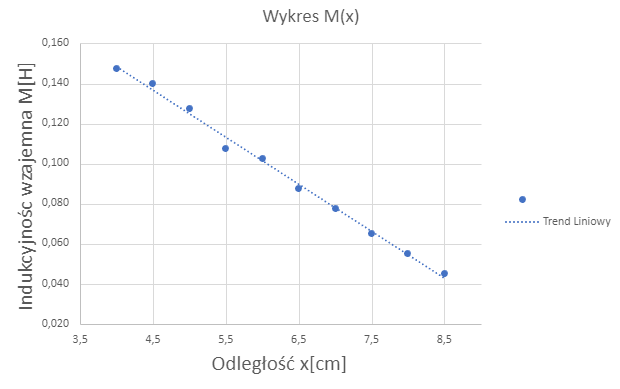
\includegraphics[scale=0.8]{cw44/wykres_cw44.png}
    \caption{Wykres zależności Indukcyjności wzajemnej M od odległości cewek x.}
    \label{fig:wykres1}
\end{figure}
\begin{figure}[H]
    \centering
    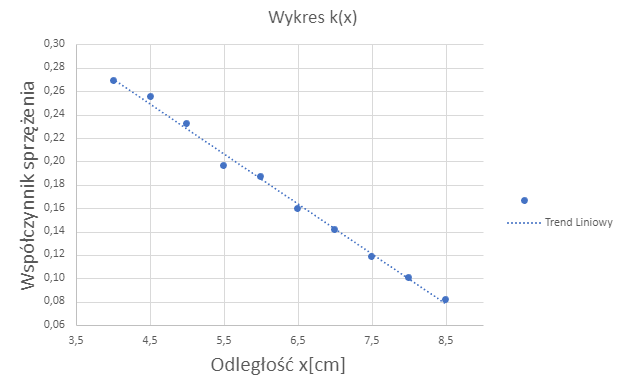
\includegraphics[scale=0.8]{cw44/wykres2_cw44.png}
    \caption{Wykres zależności współczynnika sprzężenia k od odległości cewek x.}
    \label{fig:wykres1}
\end{figure}

\section{Wnioski}
W tym ćwiczeniu zespołowi udało się zbadać zależności występujące
pomiędzy odległościami między cewkami i współczynnikami ich 
sprzężenia. Wynika z nich, że zależność ta jest liniowa, co staje
się szczególnie jasne, kiedy spojrzy się na zamieszczone wykresy.


\end{document}